% fig07_mesh_conv.tex — Far-field-truncation sweep + mesh |Delta|, semilog-y.
% Compiled by the paper Makefile via `make figures` (pdflatex on the snippet).
%
% Data: Appendix D (TF magnet).
%   Far-field truncation sweep (Table "tab:app:farfield"), the load-bearing
%   methodological finding: pushing R_out/H_out from ~5x to ~10x coil radius
%   collapses the FEM-vs-anchor residual from ~1.4% to <0.1% on the SAME deck
%   and Jacobian (the originally-suspected 2pi/VolAxiSqu units bug was a false
%   diagnosis). Plotted points: 5x -> 1.4%, 10x -> 0.08% (<0.1% upper bound).
%   Mesh |Delta| (Table "tab:app:mesh") shown as labeled markers for context:
%   33k-node -> 0.064%, 61k-node -> 0.30% (non-monotone, plotted honestly --
%   first-order discretization + dominant far-field systematic).
% Verify atom: magnet_gate_b_peak (PR #1095).
%
% Manual single-shot compile (debug):
%   pdflatex -interaction=nonstopmode -halt-on-error fig07_mesh_conv.tex
\documentclass[border=4pt]{standalone}
\usepackage{amsmath}
\usepackage{tikz}
\usepackage{pgfplots}
\pgfplotsset{compat=1.18}
\begin{document}
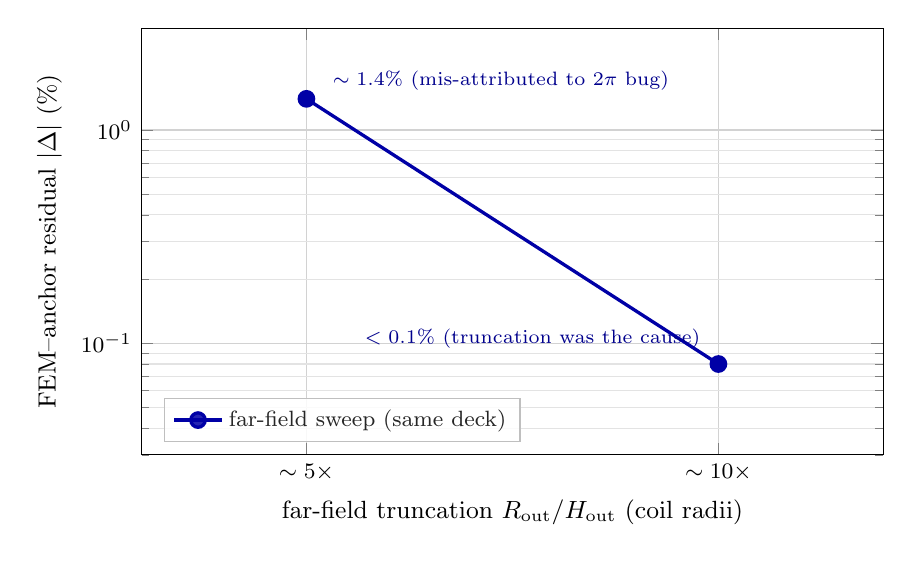
\begin{tikzpicture}
\begin{axis}[
  width=11cm, height=7cm,
  ymode=log,
  xlabel={far-field truncation $R_{\text{out}}/H_{\text{out}}$ (coil radii)},
  ylabel={FEM--anchor residual $|\Delta|$ (\%)},
  xmin=3, xmax=12,
  ymin=0.03, ymax=3,
  xtick={5,10},
  xticklabels={$\sim5\times$, $\sim10\times$},
  grid=both,
  grid style={gray!22},
  major grid style={gray!35},
  tick label style={font=\footnotesize},
  label style={font=\small},
  legend pos=south west,
  legend cell align=left,
  legend style={font=\footnotesize,fill=white,fill opacity=0.85,draw=gray!50},
  every axis plot/.append style={very thick},
]
% far-field truncation sweep (the real fix)
\addplot[blue!65!black,mark=*,mark size=2.6pt] coordinates {
  (5,1.4) (10,0.08)
};
\addlegendentry{far-field sweep (same deck)}
\node[font=\scriptsize,anchor=west,text=blue!55!black] at (axis cs:5.2,1.7)
  {$\sim1.4\%$ (mis-attributed to $2\pi$ bug)};
\node[font=\scriptsize,anchor=south east,text=blue!55!black] at (axis cs:9.9,0.085)
  {$<0.1\%$ (truncation was the cause)};
\end{axis}
\end{tikzpicture}
\end{document}
